\subsection{Road Generation}
The fundamental infrastructure of a city is the road network and, as such, it was important that the road generation would be both flexible and offer realistic results.
To generate such networks, the RoadGenerator function was designed (see Table~\ref{table:def_roadgen}).

\begin{table}[H]
  \centering
  \begin{tabular}{lllll}
    \textbf{Input} & & \textbf{Function} & & \textbf{Output} \\
    \midrule
    \textit{Terrain, PopulationMap, Markers} & $\rightarrow$ & \textbf{RoadGenerator}       & $\rightarrow$ & \textit{RoadNetwork}    \\
    \bottomrule
  \end{tabular}

  \caption{Definition of the RoadGenerator which is responsible for generating road networks.}
  \label{table:def_roadgen}
\end{table}
\vspace{-0.4cm}

This function uses the terrain to place down roads, the population map to determine where roads are needed, and input markers to form city center patterns.

Three approaches were considered when designing the road generator.
The first was based on a recursive approach where the world was divided into cells with roads placed between the cells, forming a similar structure to Voronoi Diagrams.
However, this type of algorithm did not provide realistic-looking results.
Regardless of being flexible, it was overly complicated for the purpose of creating a realistic road networks.
The second approach was search-based and would involve ML to produce structures based on data.
However, proper data appeared difficult to gather and evaluation of candidate solutions would become highly challenging.

The final approach that was decided to be used in the project involved an Agent-based generation which simulated road workers traversing the terrain.
The sole purpose of these Agents was to create roads based on different road building strategies.
Agents could also decide to branch into multiple new Agents, thus forming intersections in the road network.
Which strategy to use depends entirely on the goal of the generation, but the focus of this project has been to create a flexible base that could be extended to mimic any type of city generation.
As such, this project only includes Paris and Manhattan strategies, with the generation of main roads depending on the city strategy in order to achieve the aesthetics of the specific city type.
Paris-like cities have distinct rings within the city boundaries, while Manhattan-like cities follow a much more grid-like structure.

Furthermore, Agents may switch strategy mid-generation, be it randomly, or depending on some variables that the Agent has access to.
For example, if an Agent detected a relatively low population density, it might decide to switch to a village-type strategy that could produce smaller villages with a different layout than cities like Paris or Manhattan.

Strategies can also define the configuration of the Agent, such as step size, how many steps an Agent can take before terminating (step count), and how many times an Agent can branch.
The strategy that the Agent uses is responsible for deciding when an Agent should terminate, except for step count which is handled automatically for all strategies.

The road generator uses the city markers as input to create the initial Agents that will start creating the road network.
Each city type needs its own preset arguments for the Agents, and this was solved by assigning an Agent factory to each city type.
The goal of the Agent factory is determining starting conditions for Agents depending on the city type.

For example, in Figure~\ref{fig:road_network_paris}, the road generator started by creating a ParisAgentFactory, which takes the city position and radius as input, and spawns multiple Agents depending on random variables within the bounds of the input.
The Agents are given a Paris-like strategy, which instructs the Agents to generate rings around the city center as well as main roads extending outwards.
This particular strategy was configured to have a very aggressive branching, which in turn produces lots of intersections.

A similar, but more basic approach, was applied to the Manhattan strategy, but instead of rings, multiple straight main roads were generated (see Figure~\ref{fig:road_network_manhattan}).

\begin{figure}[H]
  \centering
  % Use two minipages to add padding for the figure and its caption
  \begin{minipage}{.45\textwidth}
    \centering
    \begin{minipage}{.9\textwidth}
      \centering
      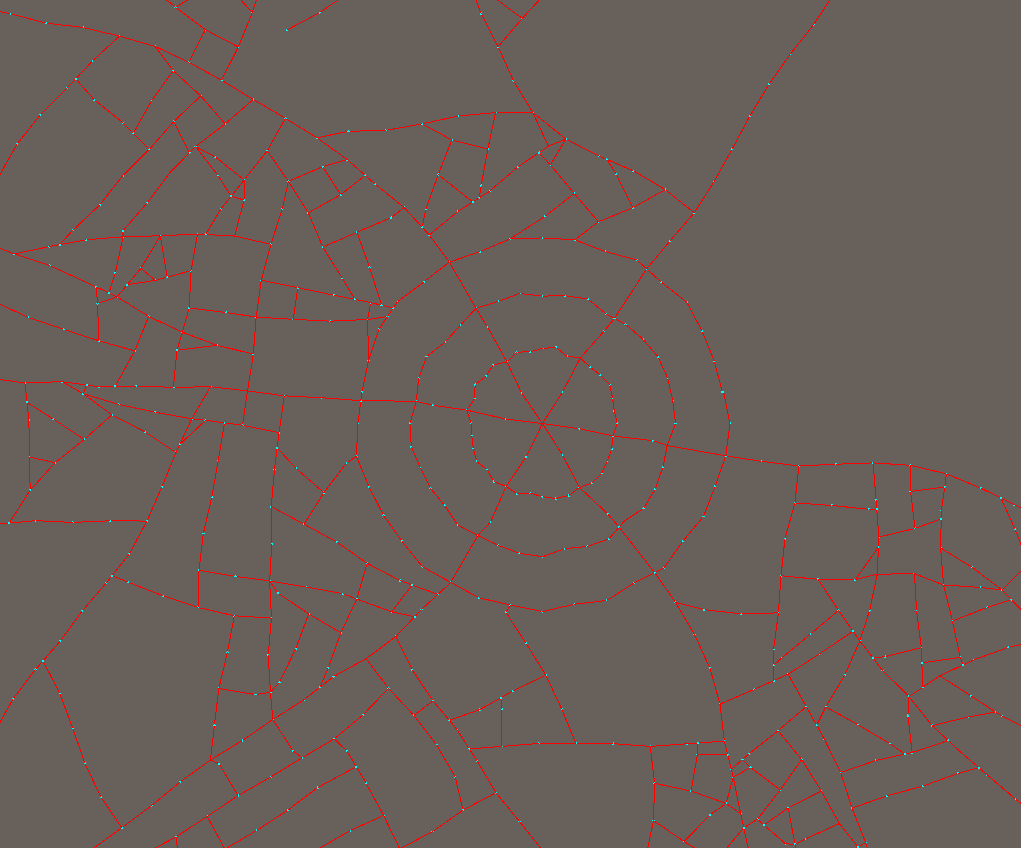
\includegraphics[width=\textwidth]{figure/road_network_paris.png}
      \caption{Example of the Paris road strategy.}
      \label{fig:road_network_paris}
    \end{minipage}
  \end{minipage}
  \begin{minipage}{.45\textwidth}
    \begin{minipage}{.9\textwidth}
      \centering
      \centering
      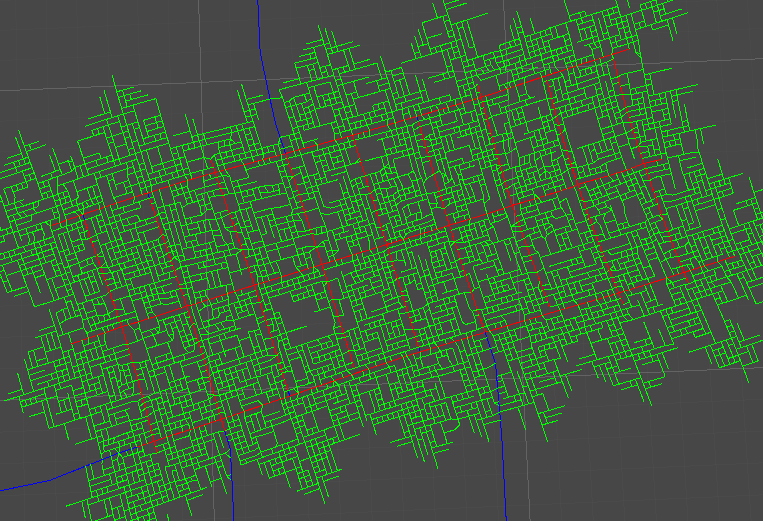
\includegraphics[width=\textwidth]{figure/road_network_manhattan.png}
      \caption{Example of the Manhattan road strategy.}
      \label{fig:road_network_manhattan}
    \end{minipage}
  \end{minipage}
\end{figure}


%% Intersection logic %%

While strategies handle how the Agent move, they do not decide how the roads should be placed.
When an Agent decides to place a road, it will attempt to find nodes in the nearby area to snap to.
If no such nodes are found, it will create a road between its previous position and its new position, and any roads that exist on the path in-between will be combined into an intersection.
Figure~\ref{fig:road_connection_cases} demonstrates the intersection created after an Agent attempts to cross another road, as well as an optimization technique making use of an R-Tree data structure \cite{wiki:R-tree}.

The R-Tree is necessary to quickly search for intersecting roads by avoiding to iterate over all nodes in the road network, or else the performance would result in an unusable application.
Each node is placed in the R-Tree with a bounding box that encapsulates each connecting node.
When two nodes are connected, the road network will search for nearby nodes that intersect with the bounding box of the new connection, as well as a snap radius.

There are a few cases where it is preferable to not create new nodes for Agents, but rather snap to nearby nodes or network edges.
The algorithm tests for four different cases, visualized in Figure~\ref{fig:road_connection_cases}.

\begin{figure}[H]
  \centering

  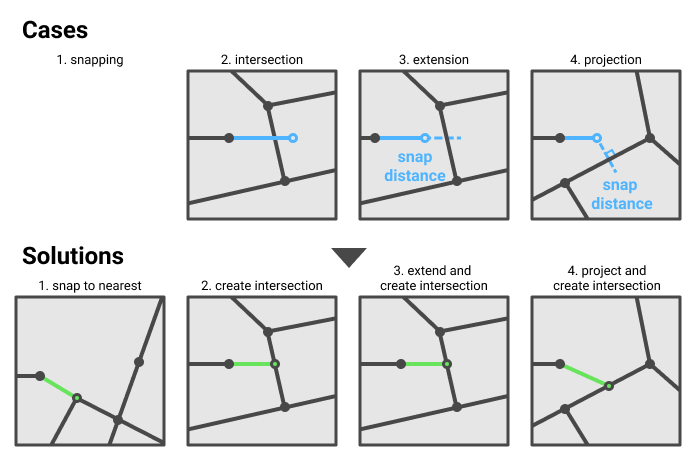
\includegraphics[width=0.8\textwidth]{figure/road_connection_cases.png}
  \caption{Four different cases that are handled in the road network connection logic.}

  \label{fig:road_connection_cases}
\end{figure}

% Move below? The caseenum should probably directly below the figure.
The solutions to the first three cases are similar to those found in the description of the snapping algorithm in the CityGen paper\cite{citygen_paper}, but these were not enough as it often happened that nodes still appeared close to roads without creating an intersection. % TODO: REFERENCE
To combat this, the solution in the fourth case was added.

\begin{CaseEnum}
  \item The algorithm searches for nodes along the path to the new node, as well as within a radius around the node.
  The distance it searches for is defined in the Agent configuration, which any strategy can define.
  If a node is found, a connection between the previous node and that node will be made, making sure to re-run the algorithm in case paths are blocking.

  \item When there is a road between the origin node and the destination node, a new node will be created, splitting the road where the intersection point is.
  The destination node is then discarded, but note that in Figure~\ref{fig:road_intersection}, the destination node was \textbf{not} discarded.
  In this project, however, the Agent will always stop at the intersection point rather than walk past it.

  \item There are cases where an Agent lands just slightly before another road, but not near enough any other nodes.
  In these cases, the best approach is attempting to extend the node forward a certain distance (the snapping distance), and check if any other roads are intersecting.
  If any are found, split the road at the intersection point and connect the origin node to the intersection node.

  \item The final case occurs when the angle of approach relative to another road is small enough that the extension in the previous case will fail because the intersection point is further away than the snapping distance.
  To solve this, the network checks if there are any roads nearby by creating a perpendicular projection onto onto those roads.
  If the distance to that projection point is within the snapping distance, the same solution is applied as in \textbf{Case 3}.
\end{CaseEnum}

First, the algorithm will search for nodes along the path to the new node, as well as a radius around the node.
The second test attempts to \textit{``extend''} the node further forward, and if it intersects with an edge, it will create an intersection there.
The last test does another intersection test, but instead of extending the node forward, it will project the node to nearby edges and create an intersection there if it is within the snap radius.


\begin{wrapfigure}[11]{r}{0.3\textwidth}
  \centering
  \raisebox{0pt}[\dimexpr\height-2\baselineskip\relax]{
    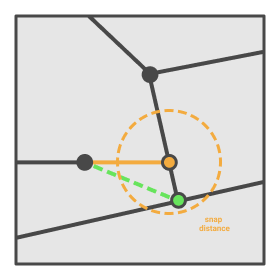
\includegraphics[width=0.26\textwidth]{figure/road_intersection_final_test.png}
  }
  \caption{Example of the test step before intersection node is created.}

  \label{fig:road_intersection_final_test}
\end{wrapfigure}

While these cases solve most of the issues in the road network and make sure Agents are not creating unnecessary roads, it is still not enough to guarantee a good-looking road network.
In cases 2, 3, and 4, one question that came up was \textit{``what happens if the node that was created at the intersection is too close to one of the nodes at the ends of the connection?''}.
The solution to this was that before the node is created and connected, it would take the point of the intersection and check for nearby nodes on the ends of the connection.
If any of those are within the snapping distance, it will snap to the nearest one instead.

%% Highways %%

Along with main roads within city bounds, RoadGenerator also produced highways that connected cities together.
The goal of highway strategies was to instruct Agents to generally move towards higher population areas.
When a suitable strategy is implemented that accomplishes this, other strategies can make use of the ability to switch Agent strategies mid-iteration.
For instance, the Paris and Manhattan strategies that were used in the project would switch the Agent strategy to a highway one once the Agent stepped outside the boundaries of the city (see Figure~\ref{fig:road_highways}).

\begin{figure}[H]
  \centering

  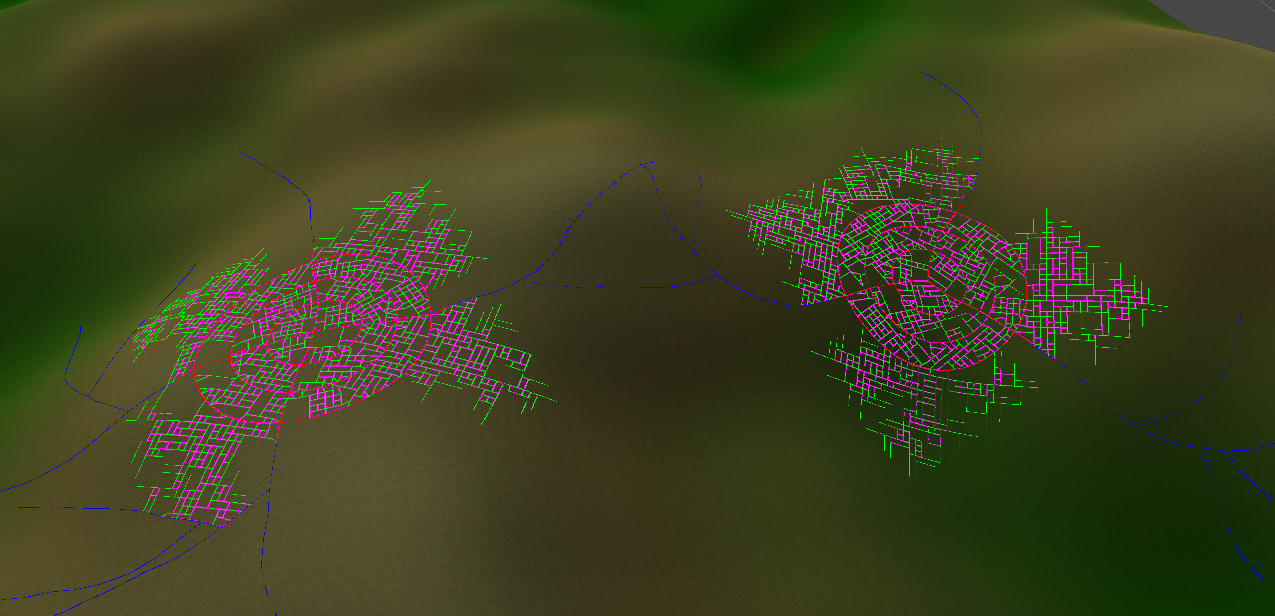
\includegraphics[width=0.8\textwidth]{figure/road_highways.png}
  \caption{Highways created outside the bounds of the city (blue lines), as well as streets (green) with blocks (purple).}

  \label{fig:road_highways}
\end{figure}

The highway strategies that were implemented into the project had a lower probability of branching than other strategies, which produced roads that were longer with fewer exits.
The aim was to produce highways that mimic the structure of highways in the real world, which this logic usually did by connecting cities together with long highways.

When the road generator is finished with the general layout of the city, the final step of generating the city roads is streets.
This was accomplished using the same road generator and Agents, but with a different strategy, which also shows the level of flexibility of the Agent-based approach.
The only difference is that these Agents start on any of the nodes in the road network and uses a street strategy, instead of starting as a city type strategy.

The base of the road generator and its strategies allows any kind of street pattern to be produced, given a suitable strategy is implemented.
In order to limit ourselves in this project, the street strategy was implemented to produce grid-like streets for all city types.
However, the configuration of the general street strategy can be configured per city type, which gives a small level of tweaking so the streets could match the city type better.

Furthermore, the street strategy (like other strategies) can watch the population map and react accordingly, either by changing direction or terminating the Agent.
Since the streets is a major part of the overall shape of the city, by letting the street strategy watch the population map, it could directly shape the city on a more detailed level than the city strategies could.
If the population density is too low, it could terminate the Agent, making sure it does not create streets and houses in an area where no population exists.
